%%%%%%%%%%%%%%%%%%%%%%%%%%%%%%%%%%%%%%%%%
% Jacobs Landscape Poster
% LaTeX Template
% Version 1.0 (29/03/13)
%
% Created by:
% Computational Physics and Biophysics Group, Jacobs University
% https://teamwork.jacobs-university.de:8443/confluence/display/CoPandBiG/LaTeX+Poster
% 
% Further modified by:
% Nathaniel Johnston (nathaniel@njohnston.ca)
%
% This template has been downloaded from:
% http://www.LaTeXTemplates.com
%
% License:
% CC BY-NC-SA 3.0 (http://creativecommons.org/licenses/by-nc-sa/3.0/)
%
%%%%%%%%%%%%%%%%%%%%%%%%%%%%%%%%%%%%%%%%%

%----------------------------------------------------------------------------------------
%	PACKAGES AND OTHER DOCUMENT CONFIGURATIONS
%----------------------------------------------------------------------------------------

\documentclass[final]{beamer}

\usepackage[size=a0,orientation=portrait,scale=1.24]{beamerposter} % Use the beamerposter package for laying out the poster

\usetheme{confposter} % Use the confposter theme supplied with this template

\setbeamercolor{block title}{fg=ngreen,bg=white} % Colors of the block titles
\setbeamercolor{block body}{fg=black,bg=white} % Colors of the body of blocks
\setbeamercolor{block alerted title}{fg=white,bg=dblue!70} % Colors of the highlighted block titles
\setbeamercolor{block alerted body}{fg=black,bg=dblue!10} % Colors of the body of highlighted blocks
% Many more colors are available for use in beamerthemeconfposter.sty

%-----------------------------------------------------------
% Define the column widths and overall poster size
% To set effective sepwid, onecolwid and twocolwid values, first choose how many columns you want and how much separation you want between columns
% In this template, the separation width chosen is 0.024 of the paper width and a 4-column layout
% onecolwid should therefore be (1-(# of columns+1)*sepwid)/# of columns e.g. (1-(4+1)*0.024)/4 = 0.22
% Set twocolwid to be (2*onecolwid)+sepwid = 0.464
% Set threecolwid to be (3*onecolwid)+2*sepwid = 0.708

\newlength{\sepwid}
\newlength{\onecolwid}
\newlength{\twocolwid}
%\newlength{\threecolwid}
%\setlength{\paperwidth}{48in} % A0 width: 46.8in
%\setlength{\paperheight}{36in} % A0 height: 33.1in
%\setlength{\sepwid}{0.024\paperwidth} % Separation width (white space) between columns
%\setlength{\onecolwid}{0.22\paperwidth} % Width of one column
%\setlength{\twocolwid}{0.464\paperwidth} % Width of two columns
%\setlength{\threecolwid}{0.708\paperwidth} % Width of three columns
\setlength{\sepwid}{0.0\paperwidth} % Separation width (white space) between columns
\setlength{\onecolwid}{0.3\paperwidth} % Width of one column
\setlength{\twocolwid}{0.6\paperwidth} % Width of two columns
\setlength{\topmargin}{-0.5in} % Reduce the top margin size
\setlength{\oddsidemargin}{-0.8in}
%-----------------------------------------------------------

\usepackage{graphbox,graphicx}  % Required for including images

\usepackage{booktabs} % Top and bottom rules for tables

\usepackage{algorithm2e}
\usepackage{amsmath}
\DeclareMathOperator*{\argmax}{argmax}

%----------------------------------------------------------------------------------------
%	TITLE SECTION 
%----------------------------------------------------------------------------------------

\title{Supervised Machine Learning for Extractive Query Based Summarisation of Biomedical Data} % Poster title

\author{Mandeep Kaur \and Diego Moll\'a} % Author(s)

\institute{Macquarie University} % Institution(s)

%----------------------------------------------------------------------------------------

\begin{document}

\addtobeamertemplate{block end}{}{\vspace*{2ex}} % White space under blocks
\addtobeamertemplate{block alerted end}{}{\vspace*{2ex}} % White space under highlighted (alert) blocks

\setlength{\belowcaptionskip}{2ex} % White space under figures
\setlength\belowdisplayshortskip{2ex} % White space under equations

\begin{frame}[t] % The whole poster is enclosed in one beamer frame

\vspace{-1cm}

\begin{columns}[t] % The whole poster consists of three major columns, the second of which is split into two columns twice - the [t] option aligns each column's content to the top

\begin{column}{\sepwid}\end{column} % Empty spacer column

\begin{column}{\onecolwid} % The first column

%----------------------------------------------------------------------------------------
%	CONTRIBUTIONS
%----------------------------------------------------------------------------------------

\begin{alertblock}{Contributions}
Within the area of query-focused extractive summarisation of biomedical data:
\begin{enumerate}
\item A comparison between classification and regression approaches.
\item A comparison of annotation methods for classification-based approaches.
\end{enumerate}

\end{alertblock}

%----------------------------------------------------------------------------------------
%	INTRODUCTION
%----------------------------------------------------------------------------------------

\begin{block}{Introduction}

We address the task of automatic query-based summarisation of biomedical text by using supervised machine learning techniques.

In addition, this research also deals with a burning issue of availability of annotated corpora for supervised learning. 

We utilised a biomedical corpus provided by the BioASQ Challenge. Each question contains, among other information:
\begin{itemize}
\item the text of the question, 
\item the question type, and 
\item a list of source documents.
\end{itemize}
The training data set contains a total of 1306 questions.
\end{block}

%-----------------------------------------------------------------------------------------
%    SUMMARISATION FRAMEWORK
%-----------------------------------------------------------------------------------------

\begin{block}{Summarisation framework}
We follow a three-stage summarisation model (Figure~\ref{fig:model}).

\begin{enumerate}
\item Pre-processing of each input sentence and question.
\item Scoring of each input sentence given the question.
\item Selection of the top $n$ scoring sentences.
\end{enumerate}
\end{block}

\begin{figure}
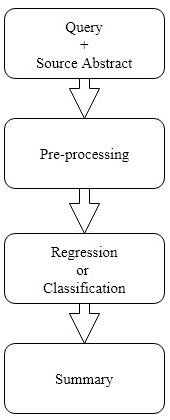
\includegraphics[width=0.5\linewidth]{model.png}
\caption{Summarisation Model\label{fig:model}}
\end{figure}

%----------------------------------------------------------------------------------------

\end{column} % End of the first column

\begin{column}{\sepwid}\end{column} % Empty spacer column

\begin{column}{\onecolwid} % Begin a column which is two columns wide (column 2)


\begin{block}{Classification / regression features}
Features used in all experiments:
\begin{itemize}
\item tf-idf vector of the candidate sentence.
\item Cosine similarity between question and candidate sentence.
\end{itemize}
\end{block}

\begin{block}{Data annotation for regression}
Each sentence of the training data is annotated with the F1 ROUGE-SU4 score of the sentence compared to the target summary. 
\end{block}

\begin{block}{Data annotation for classification}
Often the summary annotations consist of sample reference summaries, but it is not straightforward to translate this information into the target labels~1 and~0 for classification. We converted the ROUGE-SU4 score into a binary value for classification. We experimented with various thresholds:
\begin{enumerate}
\item Label three highest ROUGE-SU4 sentences with~1, the rest with~0.
\item Label all sentences with ROUGE-SU4 $>$ 0.1 with~1, the rest with~0.
\end{enumerate}
\end{block}


\begin{block}{Marcu annotation}
We also experimented with a simplification of the greedy approach proposed by \cite{Marcu:1999}. This approach takes into account the similarity between the target abstract and the entire set of sentences selected for the summary.

\vspace{3cm}

\begin{algorithm}[H]
\DontPrintSemicolon
\KwData{\\
Abstract ($A$):  The reference summary.\\ 
Text ($T$): Input text to summarise.\\
}
\KwResult{\\
Extract ($E$): A set of sentences from text which has maximum similarity to abstract}
\vspace{1ex}
    \nl $T_1, \cdots\ T_n$ = sentences from $T$\;
    \nl Stem and delete stop words from $A, T_1, \cdots\ T_n$\;
    \nl $E$ = T\;
    \nl $S = \argmax_{S'\in E}Sim(E\backslash S', A)$\;
    \nl \While{$Sim(E,A) < Sim(E\backslash S, A)$}{
                             $E = E\backslash S$\;
                             $S = \argmax_{S'\in E}Sim(E\backslash S', A)$\;}
\caption{The Marcu annotation.\label{algo}}
\end{algorithm}

\vspace{2cm}

The similarity operator $Sim(X,Y)$ is the cosine similarity between the tf-idf of $X$ and $Y$.

\end{block}

\end{column} % End of the second column

\begin{column}{\sepwid}\end{column} % Empty spacer column

\begin{column}{\onecolwid} % The third column

\begin{block}{Results}
\begin{figure}
\centering
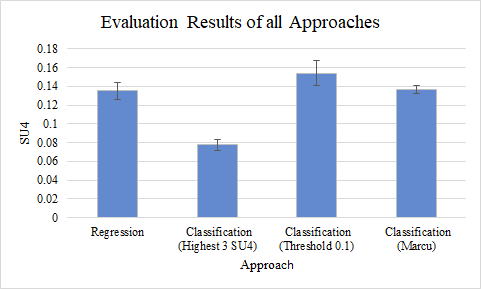
\includegraphics[width=\linewidth]{resultfig_colored.png}
\caption{Comparison of the results of the regression and three classification approaches. The results show the mean of 10-fold cross-validation, and the error bars show the standard deviation.\label{fig:all_approaches}}
\end{figure}

\end{block}

{
\setbeamercolor{block alerted title}{fg=white,bg=JungleGreen!80}
\setbeamercolor{block alerted body}{fg=black,bg=JungleGreen!10}

\begin{alertblock}{Comparison with Ouyang et al.}
A similar work by \cite{Ouyang:2011} reported better results for regression than for classification in their experiments. They used different evaluation data, features, and annotation thresholds. We therefore replicated their annotation thresholds using the BioASQ data set along with our features, and obtained an average ROUGE-S4 of 0.09. This is lower than the results of our regression approach.

Our results are therefore compatible with the results provided by \cite{Ouyang:2011} when we use their annotation thresholds for classification.
\end{alertblock}
}

\begin{alertblock}{Conclusions}

\begin{enumerate}
\item Classification can deliver better results than regression.
\item We need to be careful with the approach used to annotate the training sentences.
\end{enumerate}

\end{alertblock}

%----------------------------------------------------------------------------------------
%	REFERENCES
%----------------------------------------------------------------------------------------

\begin{block}{References}

\nocite{*} % Insert publications even if they are not cited in the poster
\small{\bibliographystyle{unsrt}
\bibliography{sample}\vspace{0.75in}}

\end{block}

%----------------------------------------------------------------------------------------
%	ACKNOWLEDGEMENTS
%----------------------------------------------------------------------------------------

\setbeamercolor{block title}{fg=red,bg=white} % Change the block title color
\vspace{-3cm}
\begin{block}{Acknowledgements}

\small{\rmfamily{Research partly funded by CSIRO's Data61}} 
\end{block}

%----------------------------------------------------------------------------------------
%	CONTACT INFORMATION
%----------------------------------------------------------------------------------------

\setbeamercolor{block alerted title}{fg=black,bg=norange} % Change the alert block title colors
\setbeamercolor{block alerted body}{fg=black,bg=white} % Change the alert block body colors

\vspace{-1cm}

\begin{alertblock}{Contact Information}

\begin{itemize}
\item Web: \href{http://comp.mq.edu.au/~diego/}{http://comp.mq.edu.au/\~{}diego/}
\item Email: \href{mailto:diego.molla-aliod@mq.edu.au}{diego.molla-aliod@mq.edu.au}
\end{itemize}

\end{alertblock}

\vspace{-1.5cm}
\begin{center}
\begin{tabular}{cc}

\includegraphics[align=t,width=0.3\linewidth]{Macquarie.png}
&
%\vspace{-3cm}

\includegraphics[align=t,width=0.3\linewidth]{data61.png}
\end{tabular}
\end{center}

\end{column}

\end{columns} % End of all the columns in the poster

\end{frame} % End of the enclosing frame

\end{document}
